\documentclass[11pt]{article}
\usepackage{amsmath}
\usepackage{sgame}
\usepackage{pstricks}
\usepackage{graphicx}		
\usepackage{hyperref}
\usepackage{natbib}

\begin{document}

\title{Solving a logistic equation with varying growth rate}
\date{}

\maketitle

%http://stackoverflow.com/questions/25001337/how-to-solve-and-plot-differential-equations-in-r

Consider a logistic growth function with a carrying capacity and a varying growth rate, where $p, \alpha, \beta \in [0,1]$.

\begin{equation}
\dot{p} = p(1-p)\frac{\beta - \alpha}{(1-p)\alpha + p\beta}
\label{original}
\end{equation}
The parameters $\alpha$ and $\beta$ determine the sign of the growth rate. If $\beta > \alpha$ then the growth rate is positive, if $\beta < \alpha$ then the growth rate is negative.

Assuming for now that $\beta > \alpha$, we know that \eqref{original} exhibits a growth rate between the following two differential equations.

\begin{equation}
\dot{p}_\alpha = p(1-p)\frac{\beta - \alpha}{\alpha}
\end{equation}

\begin{equation}
\dot{p}_\beta = p(1-p)\frac{\beta - \alpha}{\beta}
\end{equation}

In fact, we can express the original equation as a combination of these other two, where $\sigma = \frac{p\beta}{(1-p)\alpha + p \beta}$.

\begin{equation}
\dot{p} = (1-\sigma)\dot{p}_{\alpha} + \sigma\dot{p}_{\beta}
\end{equation}
Starting from an initial state with small $p$, the growth rate of \eqref{original} will initially look like $\dot{p}_\alpha$, but then become more like $\dot{p}_\beta$. That is, the growth rate will slow down over time.

We can visualize these as in Figure \ref{logistic-plot}. The growth rate of the original differential equation is always between the other two. Intuitively, this means that any solution to $\dot{p}$ will be between the solutions to $\dot{p}_\alpha$ and $\dot{p}_\beta$. 

%Interestingly as $\alpha$ and $\beta$ become closer together, the differential equation with the varying growth rate starts to look like the average of the other two.
%
%\begin{equation}
%    \lim_{\alpha \rightarrow \beta} \dot{p} = \frac{1}{2}(\dot{p}_\alpha + \dot{p}_\beta)
%\end{equation}
%I'm not entirely sure if that might be useful for determining the 

\begin{figure}
     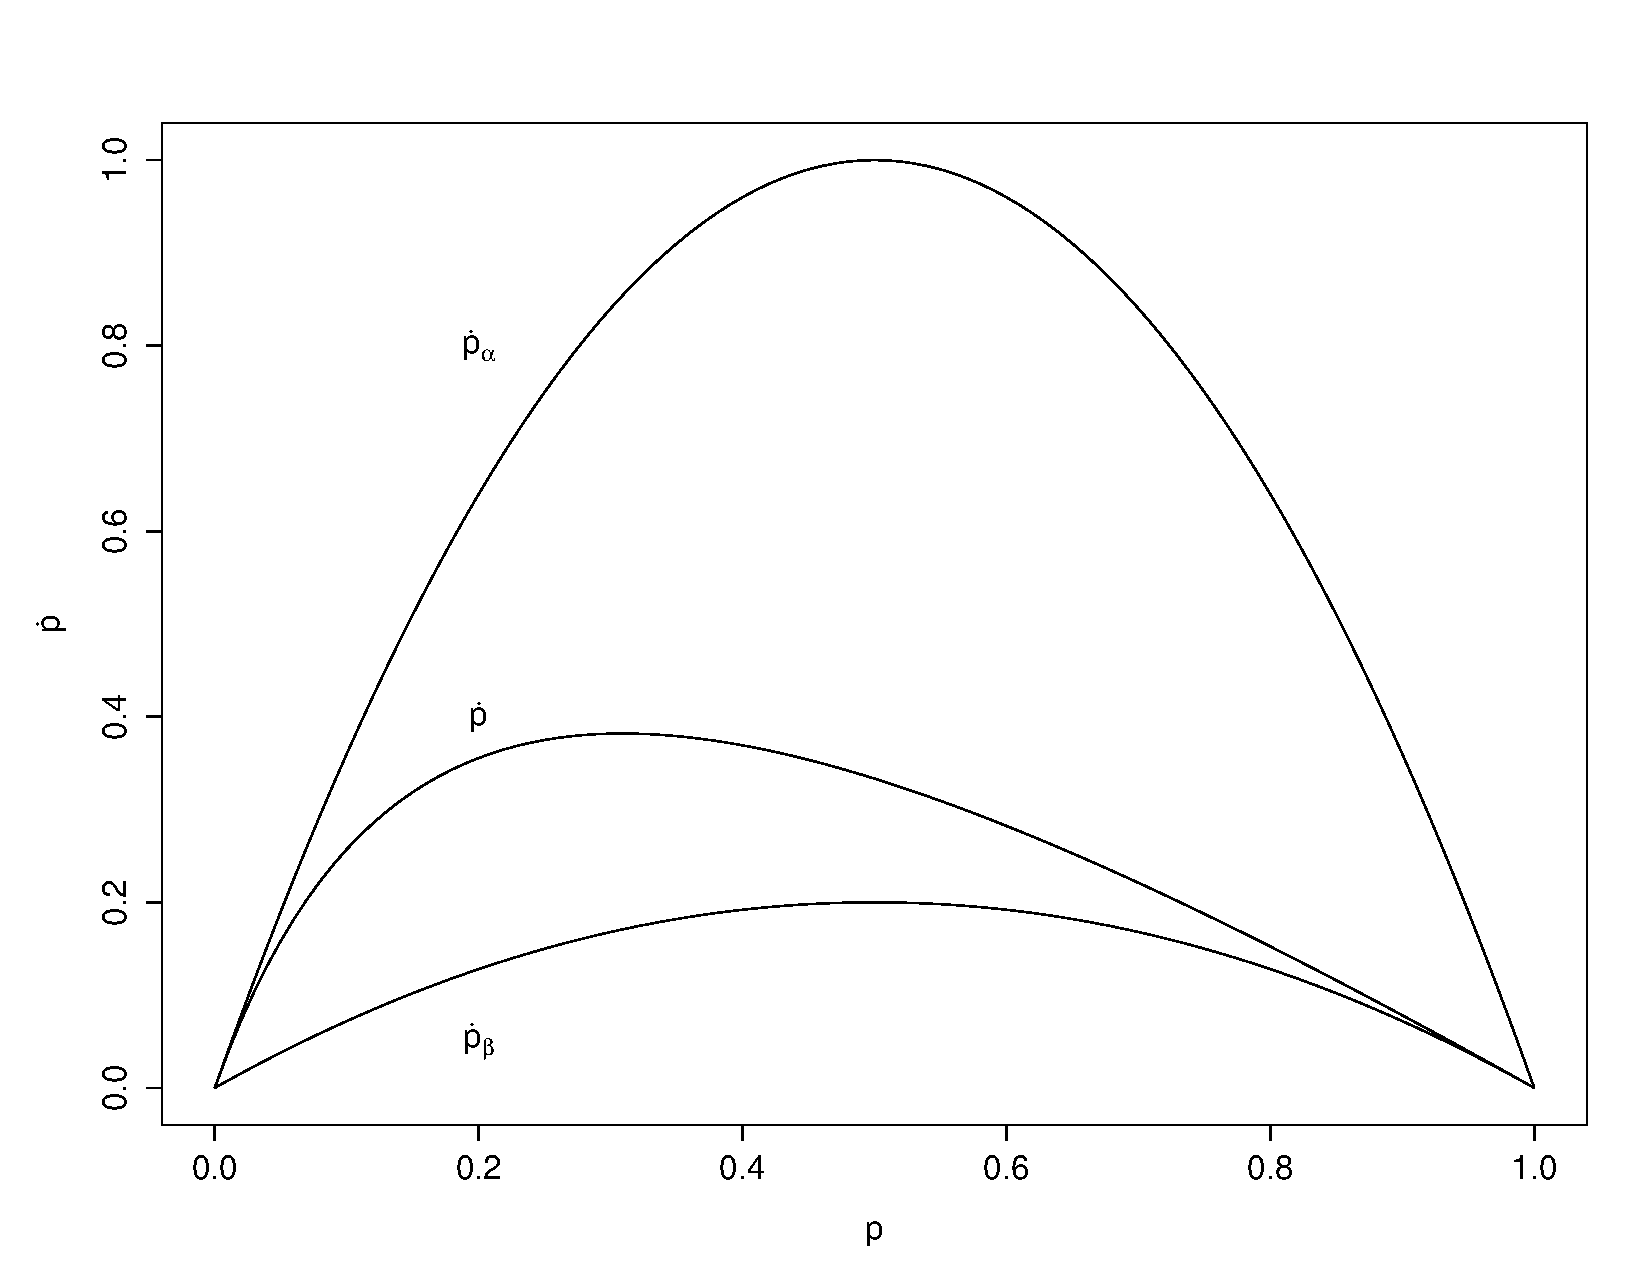
\includegraphics[width=\textwidth]{logistic-plot}
\caption{$\dot{p}_\alpha$ and $\dot{p}_\beta$ for $\alpha=.1, \beta=.5$}
\label{logistic-plot}
\end{figure}


Turning now to finding the general solution of the original differential equation, we can integrate and take antilogarithms, resulting in the following, where $K$ comes from a constant of integration. 

\begin{equation}
 \frac{p^\alpha}{(1-p)^\beta} = Ke^{(\beta - \alpha)t}
\end{equation}
Is there a means of solving for $p$? If not a closed-form solution, are there approximations that retain at least some of the information about the $\alpha$ and $\beta$? 


For a constant growth rate, $\gamma$, the solution to the logistic is the following, where $K$ results from a constant of integration.

\begin{equation}
     p_\gamma = \frac{Ke^{\gamma t}}{1 + Ke^{\gamma t}}
\end{equation}
Where $p(t_0) = p_0$, $K = \left( \frac{p_0}{1-p_o} \right)$, we have the following form for a particular solution.

\begin{equation}
     p_\gamma = \frac{\left( \frac{p_0}{1-p_o} \right)e^{\gamma t}}{1 + \left( \frac{p_0}{1-p_o} \right)e^{\gamma t}}
\end{equation}
We can visualize these two solutions, as in Figure \ref{solution-plot}.

\begin{figure}
     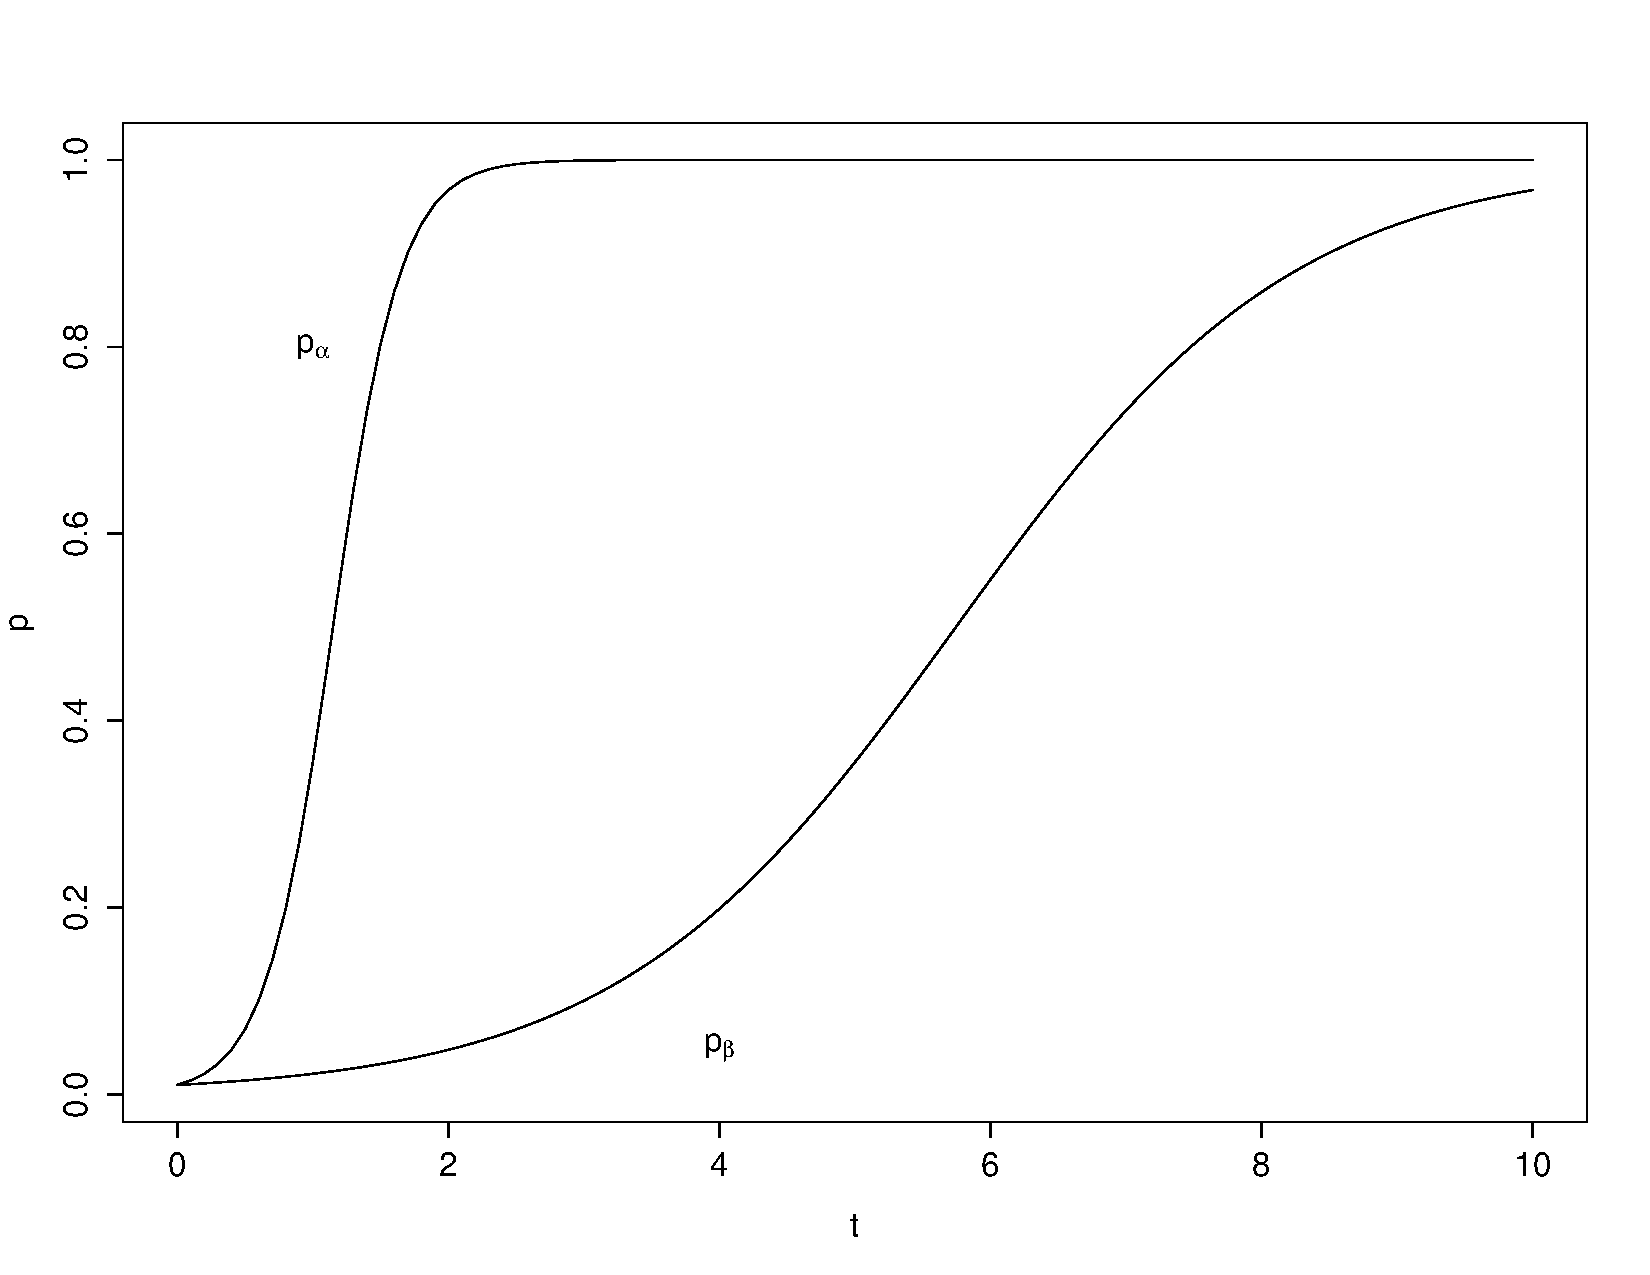
\includegraphics[width=\textwidth]{solution-plot}
\caption{$p_\alpha$ and $p_\beta$ for $p_0 = .01, \alpha=.1, \beta=.5$}
\label{solution-plot}
\end{figure}

Ideally, we'd be able to interpolate these solutions in a reasonable manner. 

% 
% $p = \frac{Ke^{\frac{\beta}{\alpha}t}}{Ke^{\frac{\beta}{\alpha}t} + e^t}$
% 
% $p = \frac{Ke^t}{Ke^t + e^{\frac{\alpha}{\beta}t}}$
% 
% If $\beta > \alpha$ then the growth rate for the first simplified equation is always greater than the second simplified equation, and the solution to the original equation will be somewhere in between these two. Is there a straightforward way to interpolate between these two solutions?

\end{document}